\section{Evaluation}
\label{sec:eval}

\begin{small}
\begin{table}[t]
	\centering
	\caption{Microarchitectural parameters}
	{\small
		\scalebox{1} {
		\begin{tabular}{|c|c|}
			\hline
			\hline
%			Core       &
%            \begin{tabular}{@{}c@{}}
%			6-wide OoO, 128-entry FTQ, 128 reservation stations, \\352-entry ROB, 128-entry load queue, 72-entry store queue
%            \end{tabular} \\

%			\hline
            \textbf{Parameter} & \textbf{Value} \\
			\hline
            Fetch & 6-wide, 128-instruction FTQ \\
			\hline
            Branch Predictor& Hashed Perceptron \\
			\hline
			Return address stack& 64 entries \\
			\hline
            Scheduler& 128 entries \\
			\hline
            Re-order buffer& 352 entries \\
			\hline
			Load queue& 128 entries \\
			\hline
			Store queue& 72 entries \\
			\hline

			L1-I &
            \begin{tabular}{@{}c@{}}
            32 KB, 8-way, \\4 cycle latency, 8 MSHRs
            \end{tabular} \\
			\hline
			L1-D &
            \begin{tabular}{@{}c@{}}
            48 KB, 12-way, \\5 cycle latency, 16 MSHRs
            \end{tabular} \\
            \hline
			L2 &
            \begin{tabular}{@{}c@{}}
            512 KB, 8-way, \\14/15 cycle latency, 32 MSHRs
            \end{tabular} \\
			\hline
			LLC &
			\begin{tabular}{@{}c@{}}
			2MB, 16-way, \\34/35 cycle latency, 64 MSHRs
			\end{tabular}\\
			\hline
			\hline
		\end{tabular}
	  }
	}
	\label{table:microParam}

\end{table}
\end{small}

%We first present the methodology used to evaluate the proposed BTB organization. Then we assess the effectiveness of BTB-X in maximizing the number of branches captured in a given storage budget. Next, we evaluate the performance benefit gained by the higher branch density of BTB-X and its sensitivity to BTB storage budget. Then, we assess how different BTB organizations fare against each other when given equal number of entries. %Finally, we analyze the power requirements of BTB-X.

\subsection{Methodology}
We use ChampSim~\cite{champsim} to evaluate the efficacy of BTB-X on server and client workload traces provided by Qualcomm for the first Instruction Prefetching Championship (IPC-1)~\cite{ipc1}. We warm up microarchitectural structures for 50M instructions and collect statistics over the next 50M. The microarchitectural parameters for the modeled processor, resembling Intel Sunny Cove~\cite{sunnycove}, are listed in \Cref{table:microParam}.

We improved two important aspects of Champsim to evaluate the baseline, state-of-the-art, and proposed BTB organizations. First, being a trace-driven simulator, Champsim detects branches by consulting the information available in the traces, rather than looking up a BTB. This essentially translates to Champsim using an ideal BTB. Therefore, we first implement a realistic conventional BTB (Conv-BTB), presented in \Cref{sec:background}, in Champsim. Second, Champsim resolves all branches in execute stage, i.e., branch mispredictions are detected and the fetch is resteered to correct path only when a mispredicted branch instruction reaches the execute stage. Such branch resolution overestimates the misprediction penalty of unconditional direct branches. This is because such branches can be resolved in the decode stage (hence, fetch can be resteered sooner) as they are always taken, thus the PC of the next instruction can be compared to the target encoded in the branch instruction to detect mispredictions. Further, taken conditional branches that miss in BTB but are correctly predicted by the direction predictor, can also be resolved in the decode stage. To do so, the fetch stage passes the direction prediction for all instructions, despite BTB hit/miss, to decode stage. If decode identifies a branch that missed in the BTB but predicted taken by the direction predictor, it resteers the fetch to the target encoded in the branch instruction, thus reducing BTB miss penalty. Given that the direction predictors are highly accurate, this optimization reduces average BTB miss penalty. Overall, we improve branch resolution so that the unconditional direct branches and the taken conditional branches that miss in BTB are resolved in the decode stage. Finally, BTB is updated at commit stage by only the taken branches (both conditional and unconditional).

%We use CACTI 7.0~\cite{cacti} to analyse the power requirements of BTB-X at 28nm technology node. The per access energy numbers obtained from CACTI are combined with the number of BTB accesses obtained from Champsim to obtain the total power consumption.

\begin{small}
\begin{table}[t!]
  \centering
  \caption{BTB-X storage requirements. The numbers in parentheses are for BTB-XC.}
  \label{table:metadata}
  \begin{tabular}{lrrr} \hline
    \textbf{Entries} & \textbf{Sets} & \textbf{Set size}
    & \textbf{Storage} \\\hline
    256(4) & 32(4) & 224(64)-bits & 0.9KB\\\hline
    512(8) & 64(8) & 224(64)-bits & 1.8KB\\\hline
    1K(16) & 128(16) & 224(64)-bits & 3.6KB\\\hline
    2K(32) & 256(32) & 224(64)-bits & 7.25KB\\\hline
    4K(64) & 512(64) & 224(64)-bits & 14.5KB\\\hline
    8K(128) & 1024(128) & 224(64)-bits & 29KB\\\hline
    16K(256) & 2048(256) & 224(64)-bits & 58KB\\\hline
  \end{tabular}
  \vspace{-0.1in}
\end{table}
\end{small}

\begin{small}
\begin{sidewaystable}
  \centering
  \caption{Number of branches in different BTB organizations at various storage budgets.}
  \label{table:btbComp}
  \begin{tabular}{cccccc} \hline
    \textbf{Storage} & \textbf{BTB-X + BTB-XC} & \textbf{PDede} & \textbf{Conv-BTB}\\\hline
    \begin{tabular}{r}
    \textbf{}\\\hline
    0.9KB\\
    1.8KB\\
    3.6KB\\
    7.25KB\\
    14.5KB\\
    29KB\\
    58KB
    \end{tabular}

    &
    \begin{tabular}{r}
    \textbf{Branches}\\\hline
    256 + 4\\
    512 + 8\\
    1K + 16\\
    2K + 32\\
    4K + 64\\
    8K + 128\\
    16K + 256
    \end{tabular}

    &
    \begin{tabular}{rrrr}
    Page-BTB budget & Main-BTB budget & Entry Size&\textbf{Branches}\\\hline
    0.078KB&0.817KB&32-bits&210\\
    0.156KB&1.645KB&32.5-bits&415\\
    0.312KB&3.3KB&33-bits&820\\
    0.625KB&6.6KB&33.5-bits&1617\\
    1.25KB&13.2KB&34-bits&3190\\
    2.5KB&26.5KB&34.5-bits&6292\\
    5KB&53KB&35-bits&12405\\
    \end{tabular}

    &
    \begin{tabular}{rr}
    Entry Size&\textbf{Branches}\\\hline
    64-bits&116\\
    64-bits&232\\
    64-bits&464\\
    64-bits&928\\
    64-bits&1856\\
    64-bits&3712\\
    64-bits&7424
    \end{tabular}\\\hline

  \end{tabular}
\end{sidewaystable}
\end{small}

\subsection{Storage breakdown}
\label{sec:storageBreak}

We first assess the number of branches different BTB organizations (Conv-BTB, PDede, and BTB-X) can accommodate in a given storage budget compared to each other. We use storage budgets required for storing 256, 512, 1K, 2K, 4K, 8K, and 16K branches in BTB-X as presented in \Cref{table:metadata}. Our calculations assume a 48-bit virtual address space and BTB-X entry compositions presented in \Cref{fig:btbx}. To double the number of entries in BTB-X, we double the number of sets while keeping the associativity same. Notice that \Cref{table:metadata} presents set size instead of entry size. This is because BTB-X features different sized entries in different ways; however, the set size remains constant.

\Cref{table:btbComp} presents the number of branches the different BTB organizations can track at different storage budgets. PDede distributes the overall BTB storage budget among its Main-BTB, Page-BTB, and Region-BTB. We follow the distribution used by its inventors\cite{pdede} to allocate the budget among different PDede BTBs as shown in \Cref{table:btbComp}. Accordingly, for 29KB storage budget, we configure PDede to use 1K Page-BTB entries and about 6K Main-BTB entries. While halving the storage budget to lower values, we halve the number of entries in the Main-BTB as well as the Page-BTB. Halving the number of Page-BTB entries reduces the number of bits required to store Page-BTB pointer in the Main-BTB. Thus, the Main-BTB entry size reduces with the reduction in storage budget. Further, we use four Region-BTB entries across all storage budgets, so Region-BTB requires a fixed storage of 0.0107KB. Also recall that PDede reserves half of the ways in a set for same-page branches while the other half can store both same-page and different-page branches. Therefore, its entries are of two different sizes. The PDede entry size shown in \Cref{table:btbComp} is the average of two sizes.


As the table shows BTB-X stores significantly more branches than any other BTB organizations. Concretely, it stores 2.24x more branches than a conventional BTB organization. Compared to PDede, BTB-X stores 1.24x more branches at 0.9KB storage budget and 1.34x more branches at 58KB storage budget. BTB-X's advantage over PDede increases with storage budget because PDede entries require more bits at higher budgets to accommodate larger Page-BTB pointers.

\begin{sidewaysfigure}
    \centering
    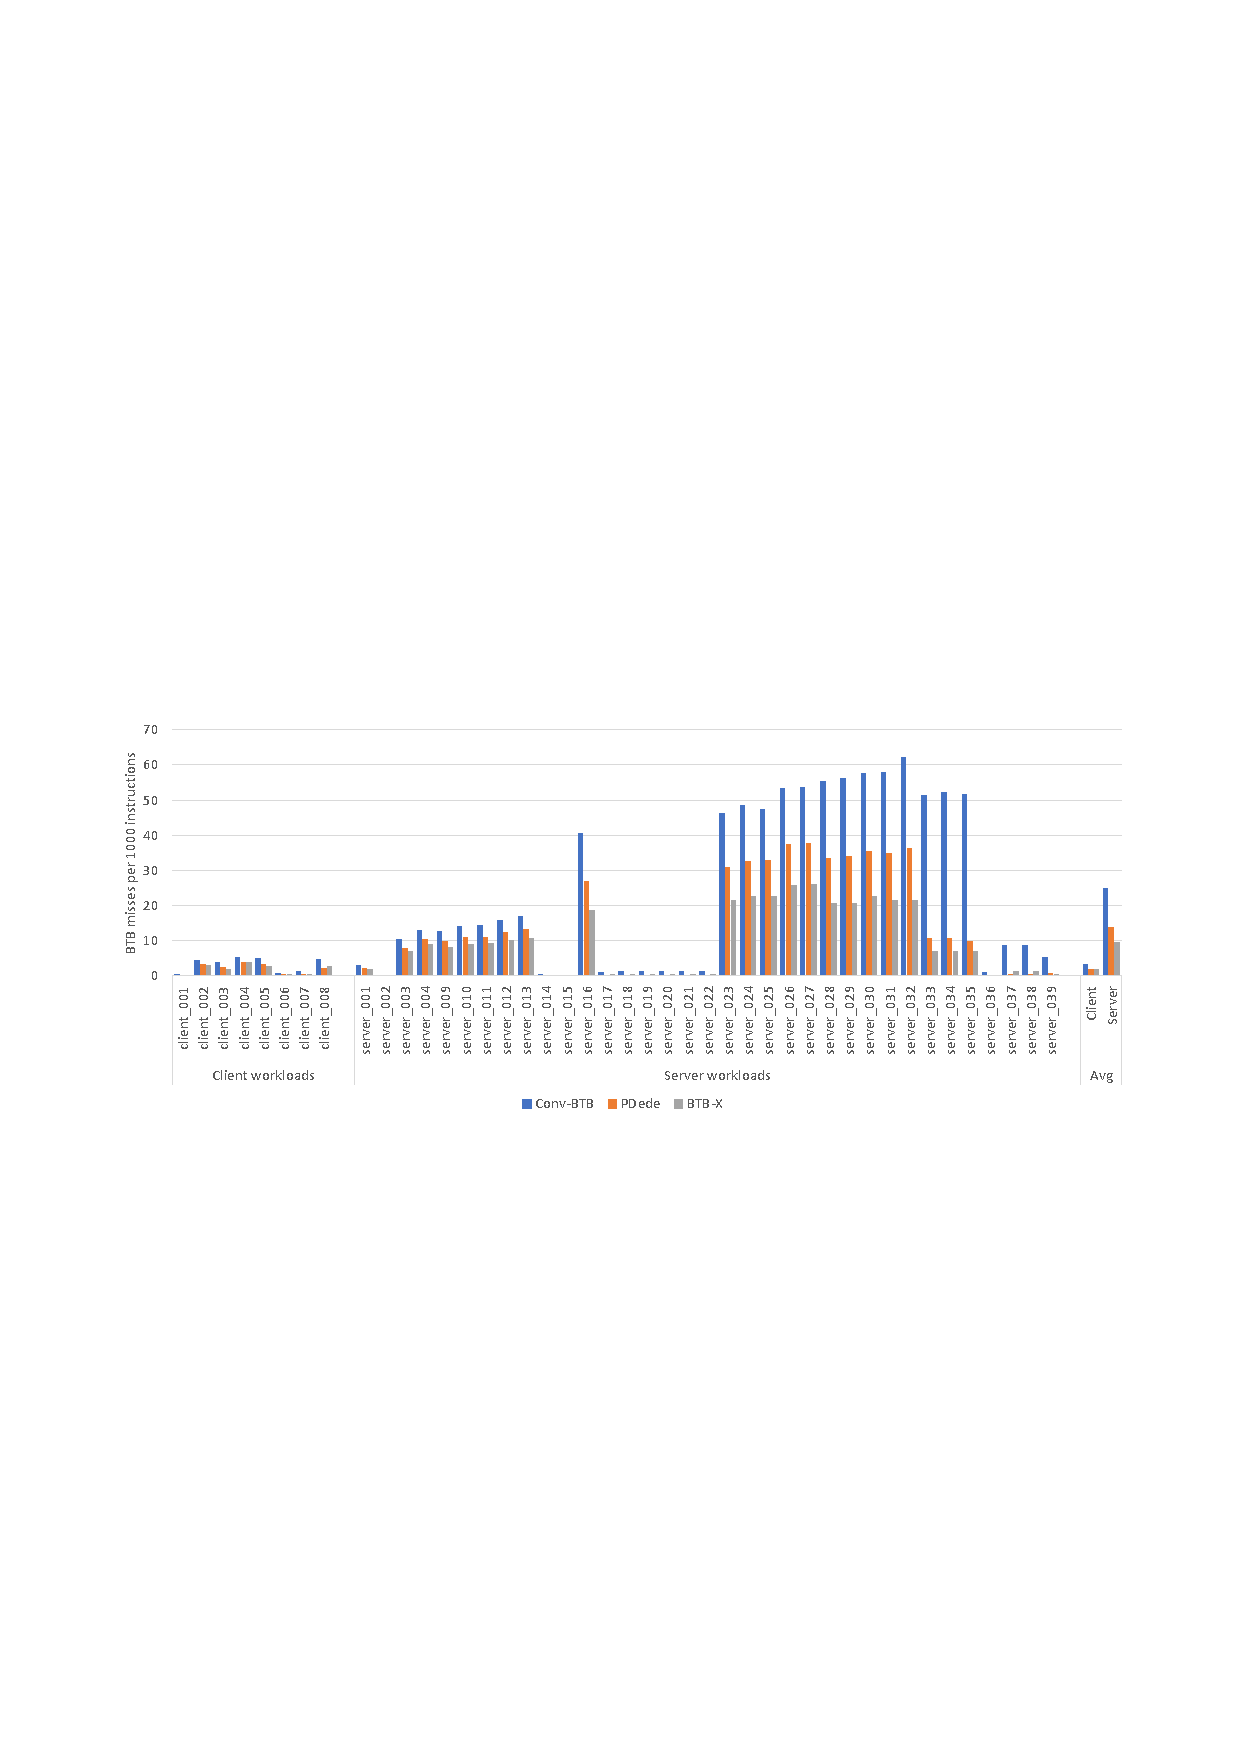
\includegraphics[width=\textwidth, trim=60 300 50 340, clip]{figures/BTBMPKI4KEQ.pdf}
    \vspace{-0.1in}
    \caption{BTB MPKI experienced by different BTB organizations.}
    \vspace{-0.2in}
    \label{fig:mpki}
\end{sidewaysfigure}

\begin{sidewaysfigure}
    \centering
    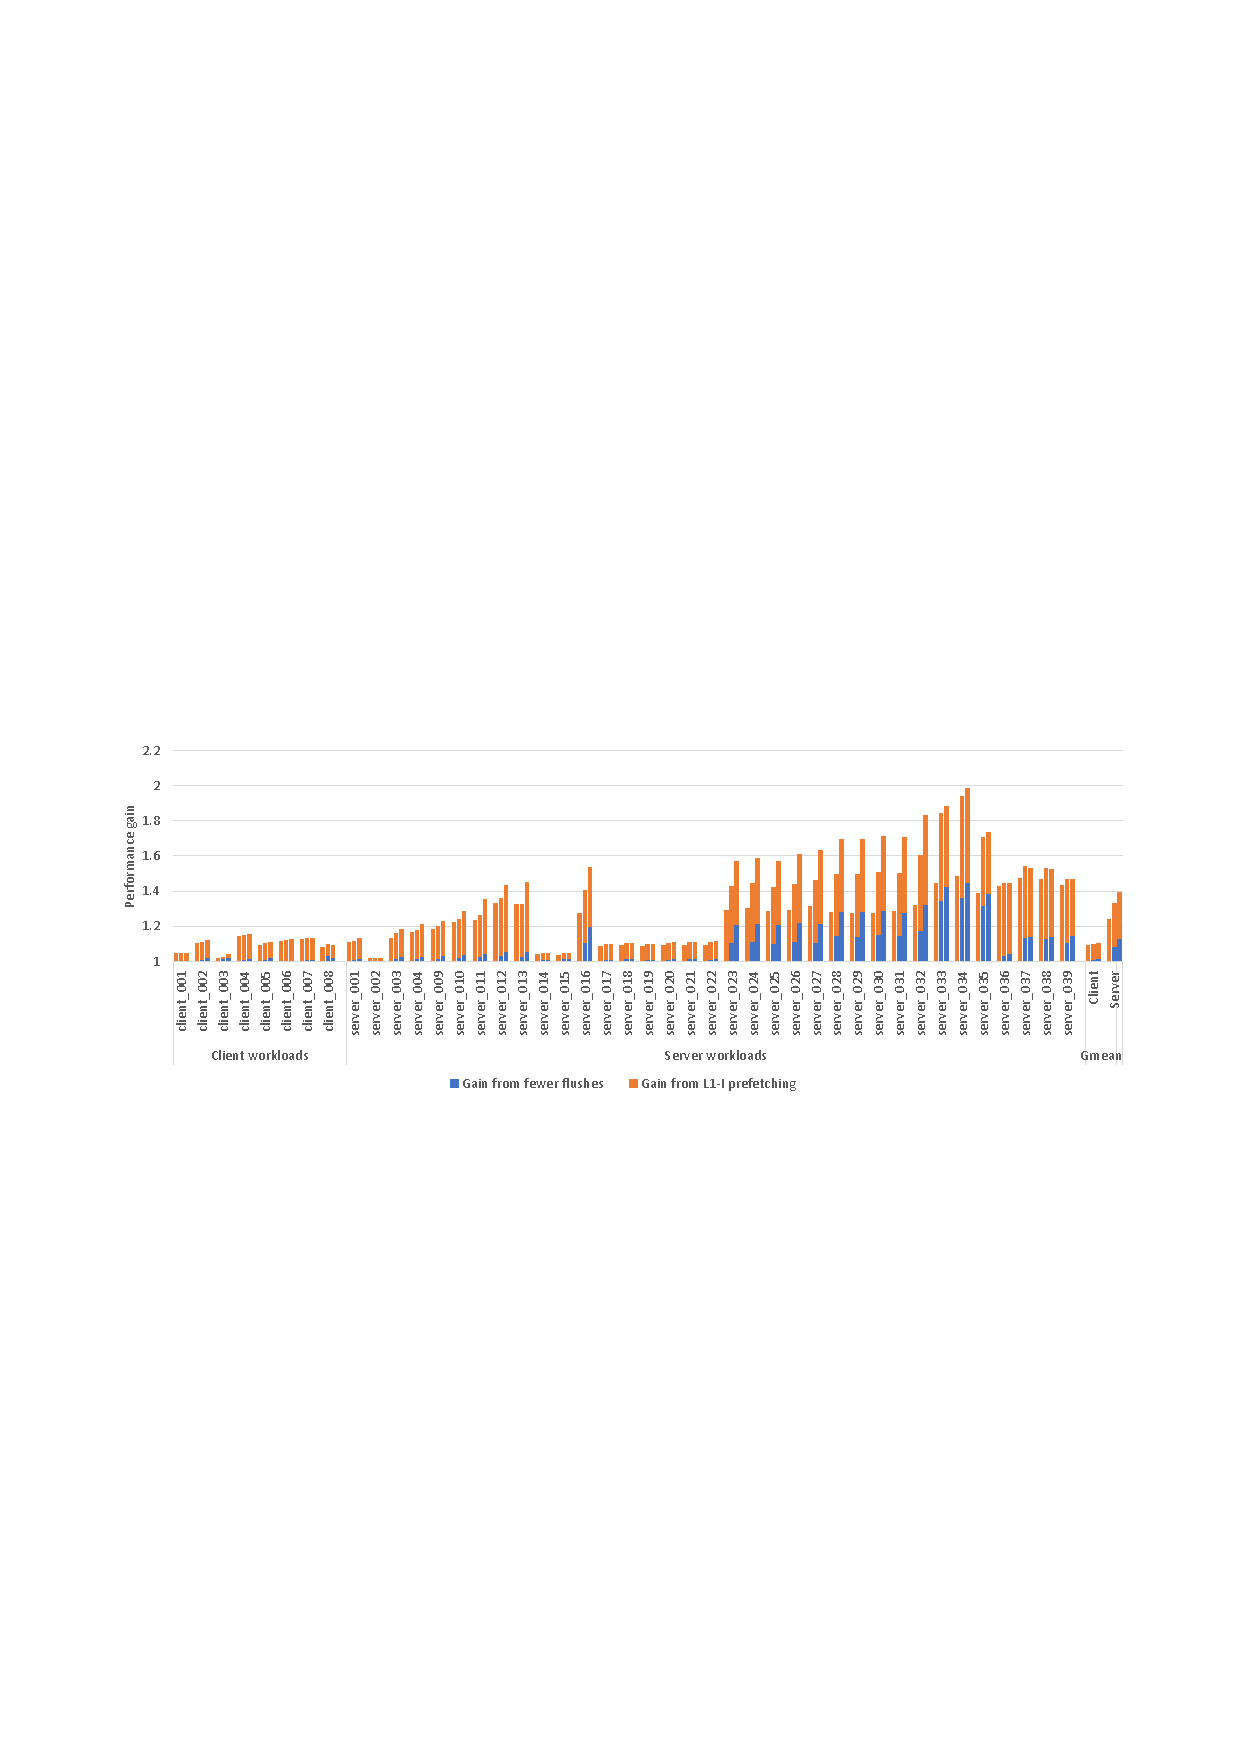
\includegraphics[width=\textwidth, trim=60 300 50 340, clip]{figures/Performance4KEQ_revised.pdf}
    \vspace{-0.1in}
    \caption{Performance gain obtained by conventional BTB (with FDIP), PDede and BTB-X (with and without FDIP) over the conventional BTB without FDIP. The three bars for each workload correspond to Conv-BTB, PDede, and BTB-X respectively.}
    \label{fig:perfAll}
\end{sidewaysfigure}

\subsection{BTB MPKI}
\label{sec:mpki}

To understand the advantage of higher BTB-X branch density, we measure misses per 1000 instructions (MPKI) that different BTB organizations incur on client and server workloads. Since BTB misses for not-taken branches do not hurt performance, we only consider the BTB misses for taken branches. For this analysis, we assume a BTB storage budget of 14.5KB that corresponds to 4160-, 3190-, and 1856-entries in BTB-X, PDede and Conv-BTB respectively. The results are presented in \Cref{fig:mpki}.

As the figure shows, server workloads experience significantly higher MPKI compared to client workload due their massive instruction and branch footprints. The figure also shows that BTB-X provides a much lower MPKI compared to both conventional BTB and PDede especially on server workload. Concretely, on average, conventional BTB incurs 25 MPKI on server workload as it stores the least amount of branches among the three organization for a given storage budget. PDede is able to lower the MPKI to 13.7 while BTB-X brings it further down to 9.5. The advantage of BTB-X over other organizations is particularly evident on very high MPKI workloads, i.e., server\_023 to server\_035, where it provides much lower MPKI compared to conventional BTB and PDede.

\subsection{Performance}
\label{sec:perfAll}

To assess how the reduced MPKI translates to performance, we compare the performance of the three BTB organizations on client and server workloads. Recall from \Cref{sec:background} that a larger BTB delivers two distinct benefits: 1) it reduces the incidence of pipeline flushes by detecting branches in the upcoming control flow and 2) it facilitates instruction prefetching when coupled with FDIP. Thus, we compare the performance gains achieved by the three BTB organizations by evaluating them with FDIP.

\Cref{fig:perfAll} presents the performance gains obtained on server and client traces. The results are normalized to the performance of the Conv-BTB without any instruction prefetching. The figure shows three bars for each workload. The first bar presents performance gain achieved by Conv-BTB when copuled with FDIP. The second and third bars present the performance gains achieved by PDede and BTB-X respectively. The PDede and BTB-X bars divide the performance gain into contributions from fewer pipeline flushes and from better instruction prefetching stemming from capturing more branches in the BTB.

Looking at the overall performance gain with instruction prefetcher (FDIP), the figure shows that BTB-X provides a geometric mean gain of 39\% over baseline on server workloads. In comparison, PDede and Conv-BTB deliver a performance gain of only 33\% and 24\% on these workloads. Looking at individual workloads, BTB-X comprehensively outperforms PDede and Conv-BTB on server\_023 to sever\_32. For example, on server\_032, BTB-X provides 83\% speedup over baseline whereas PDede and Conv-BTB achieve only 60\% and 32\% performance gain. This is because the branch working set of these workloads starts to fit in BTB-X due to its higher branch capacity. As a result, BTB MPKI lowers which not only reduces pipeline flushes and but also keeps FDIP on correct prefetch path for longer intervals.

Looking at the results without instruction prefetcher, \Cref{fig:perfAll} shows that BTB-X provides 13\% performance gain over the baseline Conv-BTB whereas PDede is achieves 8\% gain. On individual workloads, BTB-X achieves significantly high gain over Conv-BTB and PDede on workloads from server\_23 to server\_32 even without FDIP. \Cref{fig:perfAll} also shows the FDIP by itself performs better with more number of BTB entries. For example, on server\_32 FDIP with Conv-BTB provides 32\% performance gain. With PDede, the performance gain from prefetching increases to 42\% and with BTB-X it further increases to 51\%.


\begin{small}
\begin{table}[t!]
\centering
\caption{Energy requirements of different BTB designs.}
\label{tab:energy}
%     \begin{adjustbox}{width=\textwidth,center}
    % \begin{adjustbox}{center}
        \begin{tabular}{llrrr} \hline
            \textbf{BTB} & \textbf{Access Type} & \textbf{Energy} & \textbf{\#Accesses} & \textbf{Energy}\\
             &  & \textbf{(Per access)} &  & \textbf{(Total)}\\\hline
            \multirow{3}{*}{Conv-BTB} & \multicolumn{1}{l}{Read} & \multicolumn{1}{r}{13.2pJ} & \multicolumn{1}{r}{1.60E+08} & \multicolumn{1}{r}{2122µJ}\\\cline{2-5}
                                      & \multicolumn{1}{l}{Write} & \multicolumn{1}{r}{25.2pJ} & \multicolumn{1}{r}{4.36E+06} & \multicolumn{1}{r}{110µJ}\\\cline{2-5}
                                      & \multicolumn{1}{l}{\textbf{Total Energy}} & \multicolumn{1}{r}{} & \multicolumn{1}{r}{} & \multicolumn{1}{r}{\textbf{2232µJ}}\\\hline

            \multirow{6}{*}{PDede} & \multicolumn{1}{l}{Main-BTB Read} & \multicolumn{1}{r}{8.4pJ} & \multicolumn{1}{r}{1.24E+08} & \multicolumn{1}{r}{1047µJ}\\\cline{2-5}
                                 & \multicolumn{1}{l}{Main-BTB Write} & \multicolumn{1}{r}{12.5pJ} & \multicolumn{1}{r}{5.74E+05} & \multicolumn{1}{r}{7µJ}\\\cline{2-5}
                                 & \multicolumn{1}{l}{Page-BTB Read} & \multicolumn{1}{r}{0.9pJ} & \multicolumn{1}{r}{2.01E+06} & \multicolumn{1}{r}{2µJ}\\\cline{2-5}
                                 & \multicolumn{1}{l}{Page-BTB Write} & \multicolumn{1}{r}{0.8pJ} & \multicolumn{1}{r}{2.04E+04} & \multicolumn{1}{r}{0.02µJ}\\\cline{2-5}
                                 & \multicolumn{1}{l}{Page-BTB Search} & \multicolumn{1}{r}{6.2pJ} & \multicolumn{1}{r}{2.14E+05} & \multicolumn{1}{r}{2µJ}\\\cline{2-5}
                                 & \multicolumn{1}{l}{\textbf{Total Energy}} & \multicolumn{1}{r}{} & \multicolumn{1}{r}{} & \multicolumn{1}{r}{\textbf{1058µJ}}\\\hline

            \multirow{3}{*}{BTB-X} & \multicolumn{1}{l}{Read} & \multicolumn{1}{r}{8.5pJ} & \multicolumn{1}{r}{1.16E+08} & \multicolumn{1}{r}{994µJ}\\\cline{2-5}
                                 & \multicolumn{1}{l}{Write} & \multicolumn{1}{r}{11.4pJ} & \multicolumn{1}{r}{4.03E+05} & \multicolumn{1}{r}{5µJ}\\\cline{2-5}
                                 & \multicolumn{1}{l}{\textbf{Total Energy}} & \multicolumn{1}{r}{} & \multicolumn{1}{r}{} & \multicolumn{1}{r}{\textbf{999µJ}}\\\hline

        \end{tabular}
%     \end{adjustbox}
\end{table}
\end{small}


These results show that by accommodating more branches in a given storage budget, BTB-X not only reduces pipeline flushes but also improves instruction prefetching, both lead to better performance.

\begin{figure*}
    \centering
    \begin{subfigure}[t]{0.935\columnwidth}
        \centering
        %\includegraphics[width=\textwidth]{imgs/ShotgunBTB_V2.pdf}
        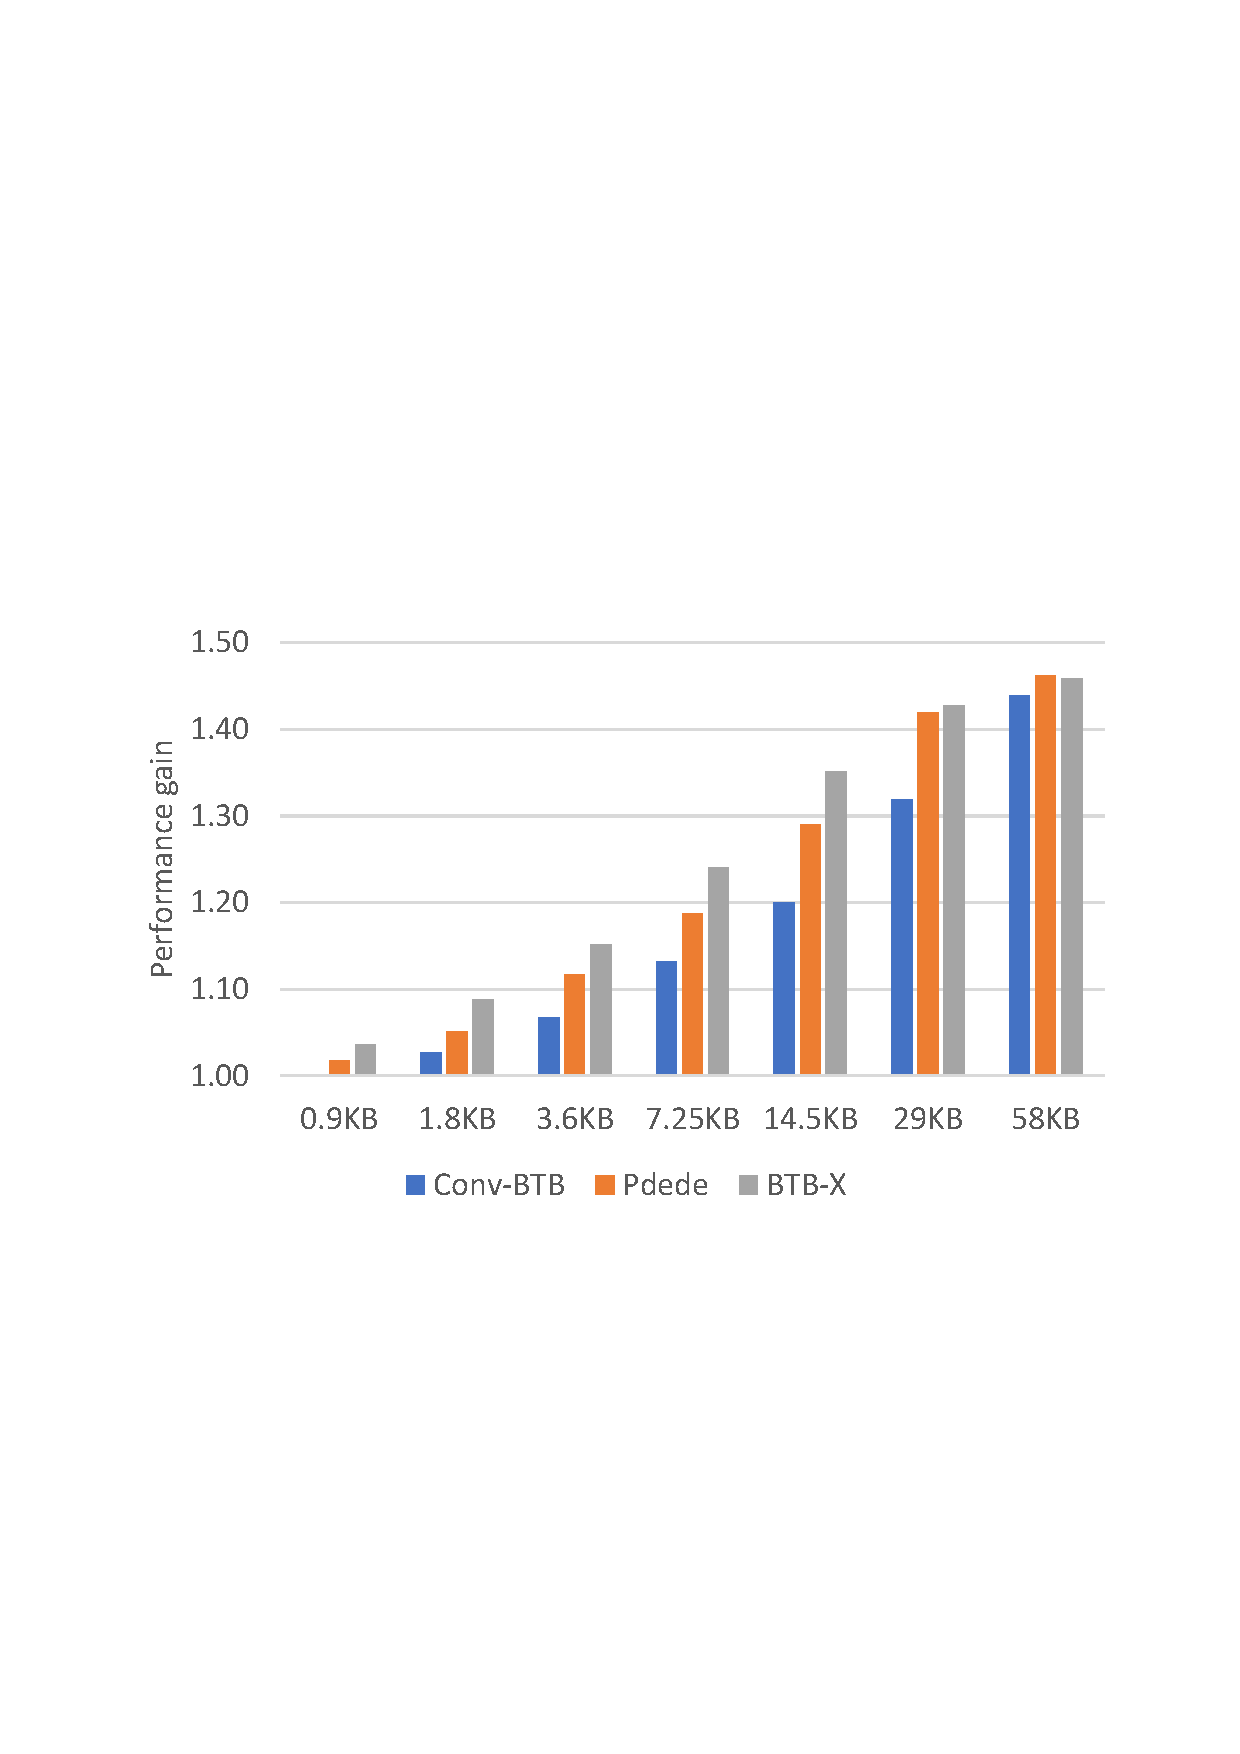
\includegraphics[width=0.935\columnwidth, trim=70 235 60 250, clip]{figures/ISOStorage_server_revised.pdf}
        \caption{Server workloads}
        \label{fig:serverPerf}
    \end{subfigure}
    ~ %add desired spacing between images, e. g. ~, \quad, \qquad, \hfill etc.
      %(or a blank line to force the subfigure onto a new line)
    \begin{subfigure}[t]{0.935\columnwidth}
        \centering
        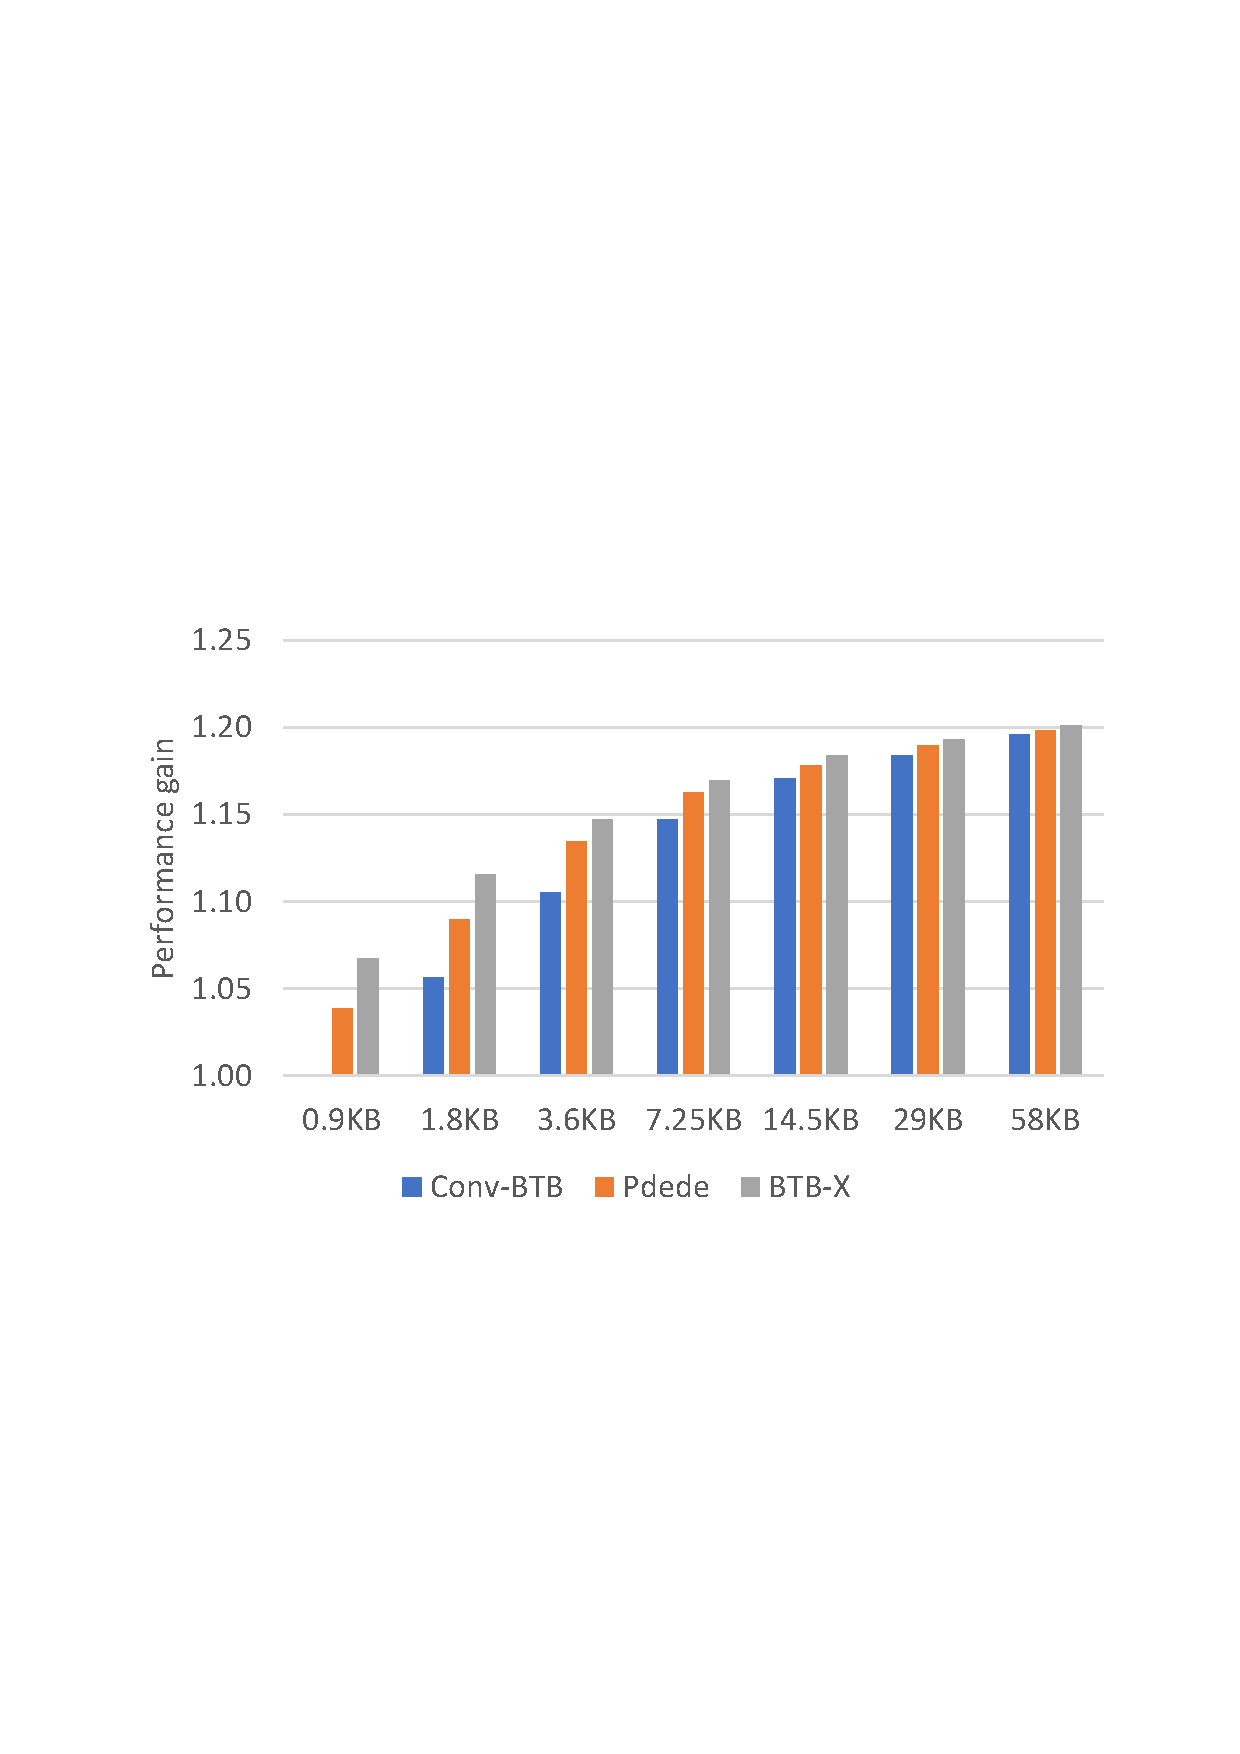
\includegraphics[width=0.935\columnwidth, trim=70 235 60 250, clip]{figures/ISOStorage_client_revised.pdf}
        \caption{Client workloads}
        \label{fig:clientPerf}
    \end{subfigure}
    \caption{Performance gains for conventional BTB, PDede, and BTB-X on (a) \textbf{server} and (b) \textbf{client} workloads over a conventional BTB with 0.9KB storage budget. X-axis label is storage requirements of 256-, 512-, 1K-, 2K-, 4K-, 8K-, and 16K-entry BTB-X.}\label{fig:perf}
\end{figure*}

Finally, \Cref{fig:perfAll} shows that all three BTB organizations perform similar on client workloads. This is because their branch working sets mostly fit in the baseline Conv-BTB and the additional entries in PDede and BTB-X do not bring much performance benefit.

\subsection{Energy and delay analysis}

We use Cacti 7.0~\cite{cacti} to analyze the energy requirements and access latencies of Conv-BTB, PDede, and BTB-X at 22 nm, which is the most recent technology node supported by Cacti. For this analysis we assume the same storage budget, i.e. 14.5KB, as used in \Cref{sec:perfAll} for the performance analysis.

\subsubsection{Energy requirements}
\Cref{tab:energy} shows the per access read and write energy requirements of different BTB designs. As the table shows, BTB-X and PDede's Main-BTB incur very similar per access read and write energy cost. However, in addition to Main-BTB, PDede also needs to access Page-BTB for different-page branches, i.e., the branches that have their targets in a different page than the branches themselves. Further, the Page-BTB needs to be searched on a BTB write to check if the target page number is already in Page-BTB or not. Consequently, PDede's per access read and write energy for different page branches reaches 9.3 pico Joules (pJ) and 19.5 pJ, respectively, compared to 8.5pJ and 11.4 pJ of BTB-X. PDede also features a Region-BTB; however, its energy requirements are negligible and, thus, not shown in \Cref{tab:energy}. Finally, Conv-BTB's per access energy cost is significantly higher than BTB-X as its each read and write access requires 13.2pJ and 25.2pJ respectively.

\Cref{tab:energy} also shows the number of read/write accesses, averaged across the workloads, and the total energy consumption. Despite very similar per access energy cost, PDede' Main-BTB consumes considerably higher energy than BTB-X. This is because PDede often goes on the wrong execution path due to its higher MPKI. These additional wrong path BTB accesses, reflected in higher BTB reads in \Cref{tab:energy}, result in higher energy consumption. Further, PDede needs to handle more BTB writes than BTB-X because it holds fewer branches, which results in frequent replacements. Thus, the total energy consumption of PDede reaches 1058µJ compared to 999µJ of BTB-X. Finally, the energy requirements of Conv-BTB are significantly higher, 2232µJ, than BTB-X because of higher per access energy and higher number of total accesses.

Overall, this analysis shows that BTB-X not only delivers better performance than PDede but also consumes less energy, thus providing much better energy efficiency.

\subsubsection{Access Latency}
Our analysis shows that the Conv-BTB requires about 0.36ns to complete an access. As discussed in \Cref{sec:pdedearch}, PDede's access latency is the sum of Main-BTB and Page-BTB access latencies as these two structures are accessed sequentially. Our analysis shows that the Main-BTB and Page-BTB accesses require 0.34ns and 0.13ns, respectively, thus resulting in an overall PDede access latency of 0.47ns which is considerably higher than Conv-BTB latency. To address this, PDede employs multi-cycle BTB accesses: the Main-BTB is accessed in the first cycle, and the Page-BTB is accessed in the next cycle only if the branch is predicted to be taken and it's target is in a different page than the branch. Thus, the same page branches need one cycle and the taken different page branches need two cycles to get their target address from PDede. Finally, our analysis shows that a BTB-X access takes only 0.33ns. In summary, this analysis shows that BTB-X provides better storage efficiency without any adverse effects on the access latency.


\subsection{Performance variation with BTB storage budget}

%\begin{figure*}
%    \centering
%    \begin{subfigure}[t]{0.935\columnwidth}
%        \centering
        %\includegraphics[width=\textwidth]{imgs/ShotgunBTB_V2.pdf}
%        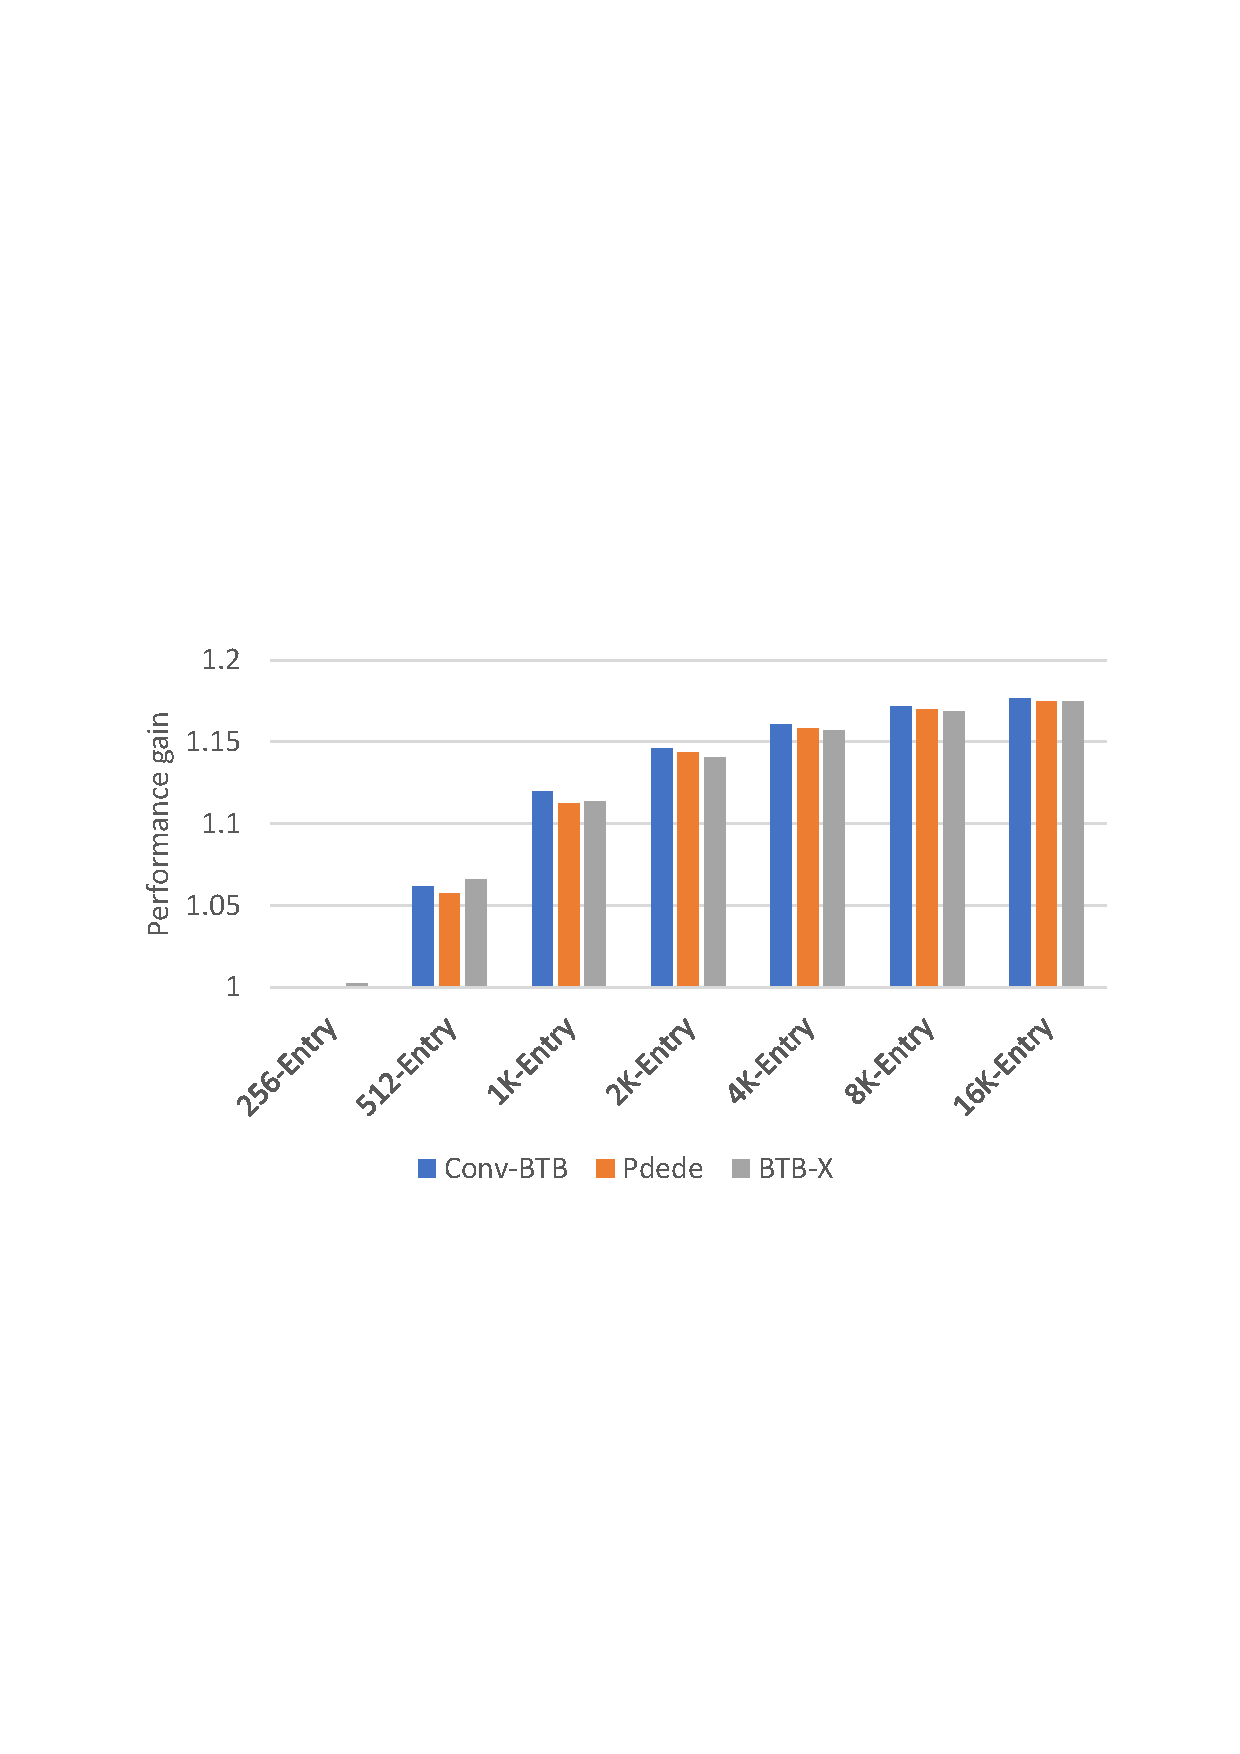
\includegraphics[width=0.935\columnwidth, trim=70 235 60 250, clip]{figures/ISOEntries-Server.pdf}
%        \caption{Server workloads}
%        \label{fig:serverPerfISOEntry}
%    \end{subfigure}
%    ~ %add desired spacing between images, e. g. ~, \quad, \qquad, \hfill etc.
      %(or a blank line to force the subfigure onto a new line)
%    \begin{subfigure}[t]{0.935\columnwidth}
%        \centering
%        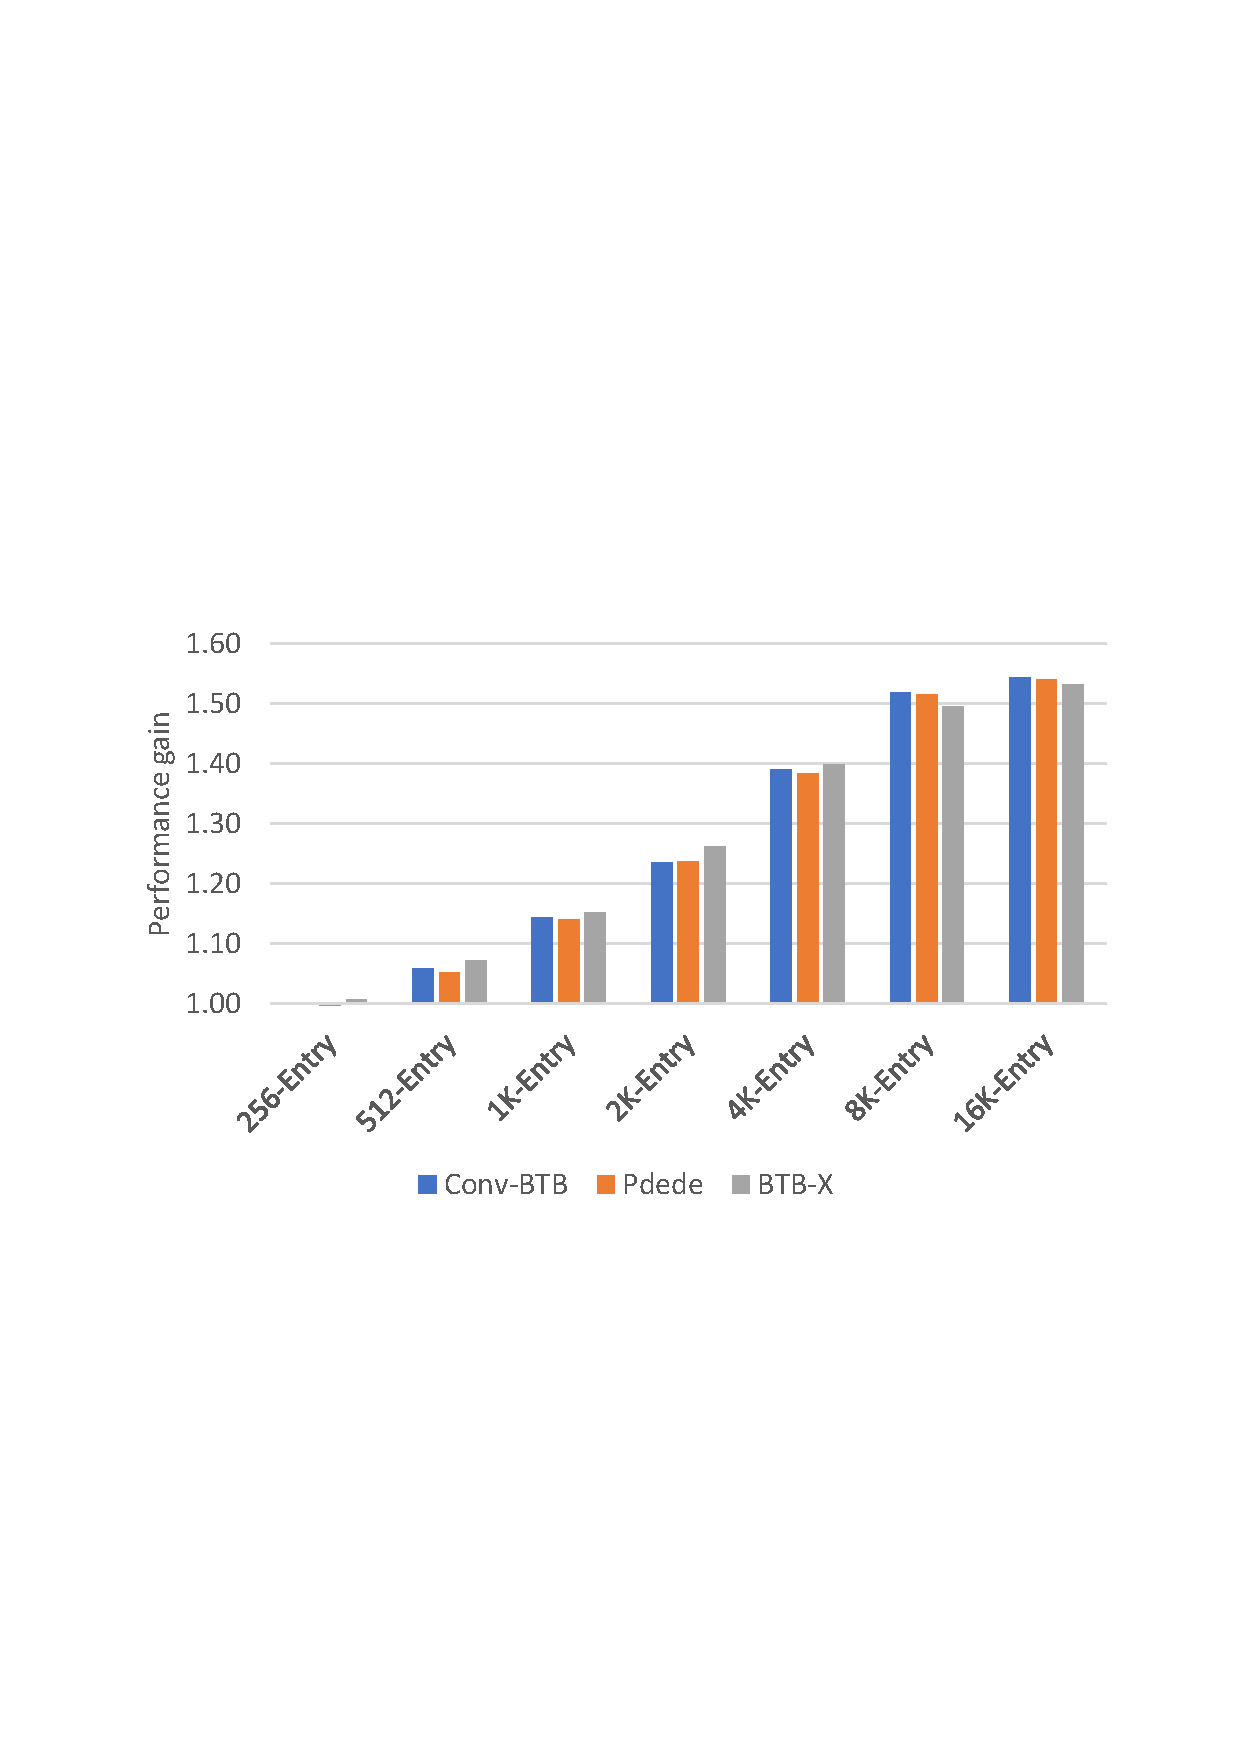
\includegraphics[width=0.935\columnwidth, trim=70 235 60 250, clip]{figures/ISOEntries-Client.pdf}
%        \caption{Client workloads}
%        \label{fig:clientPerfISOEntry}
%    \end{subfigure}
%    \caption{Performance gains for conventional BTB, PDede, and BTB-X on (a) \textbf{server} and (b) \textbf{client} workloads, over a conventional BTB with 256 entries, when all BTBs are given equal number of entries. }\label{fig:perfISOEntry}
%\end{figure*}

To further understand the performance advantage of BTB-X over PDede and Conv-BTB, we compare their performances across different storage budgets. \Cref{fig:perf} presents the performance gains obtained on server and client workloads. The results are normalized to the performance of Conv-BTB with 0.9KB storage budget. Instruction prefetching is enabled in all designs including baseline.

As the figure shows, on server workloads, BTB-X provides significantly higher performance than the Conv-BTB and PDede for equal storage budgets of up to 29KB and 14.5KB respectively. The performance advantage of BTB-X is pronounced on server traces whose large instruction footprints pressure the BTB and L1-I. For instance, BTB-X provides 35\% performance gain over the baseline compared to 29\% and 20\% of PDede and Conv-BTB respectively at 14.5KB budget. At large BTB storage budgets, the branch working sets of many workloads start to fit in the available BTB capacity, at which point the performance gap between BTB-X and the other two designs diminishes. Also, the performance gap between the three BTB organizations levels off earlier on client trace due to their smaller instruction working sets.

A key take-away from this figure is that BTB-X outperforms the conventional BTB even when it is given just half the storage budget of its conventional counterpart. For example, in \Cref{fig:serverPerf}, the Conv-BTB improves performance by 20\% with a 14.5KB budget whereas BTB-X provides a 24\% improvement with just 7.25KB. The reason for this phenomenon is that BTB-X accommodates 2.24x more entries than Conv-BTB of equal storage budget; thus, halving BTB-X's budget still gives a slight capacity advantage over Conv-BTB.

%\subsection{Performance with equal number of entries} Having analyzed ISO-storage performance, we now assess how different BTB organizations perform when given equal number of entries. Both PDede and BTB-X place restrictions on where an entry can be allocated in the BTB. For example, different-page branches in PDede can be allocated in only half of the available ways as the other half is reserved exclusively for same-page branches. Similarly, BTB-X entries are allocated based on the number of bits required for storing target offset and the offset bits available in the ways. In contrast, Conv-BTB provides full freedom in allocating any branch to any of the ways. This study will the performance penalty of restricting the branches to particular entries.

%\Cref{fig:perfISOEntry} presents the performance of three BTB designs across different number of BTB entries. The results are normalized to 256-entry Conv-BTB and instruction prefetching is enabled in all designs. As the figure shows, all BTB designs perform very similar to each other with little performance variations. These variations stem from the fact that different BTB organization are likely to hold slightly different branches, due to the restriction on branch allocation, and that different branches have different misprediction penalty. For example, unconditional direct branches can be resolved in decode stage, thus having a smaller misprediction penalty than conditional branches that are resolved in execute stage. Further, different conditional branch themselves have different latencies depending upon how quickly their dependencies can be resolved.

%Further, BTB-X implicitly favors small offset branches in BTB over large offset branches because small offset branches can be placed in more number of ways than large offset ones. As the majority of dynamically executed branches have short offsets, favoring them in a small BTB is likely to provide better hit rate and performance. However, as the number of BTB entries grow, branch working set starts to fit in BTB, so prioritizing short offset branches loses its benefits. On the contrary, having fewer entries to place large offset branches is likely to hurt performance.


\subsection{Analyzing target offset distribution in more workloads}

\begin{figure}
\centering
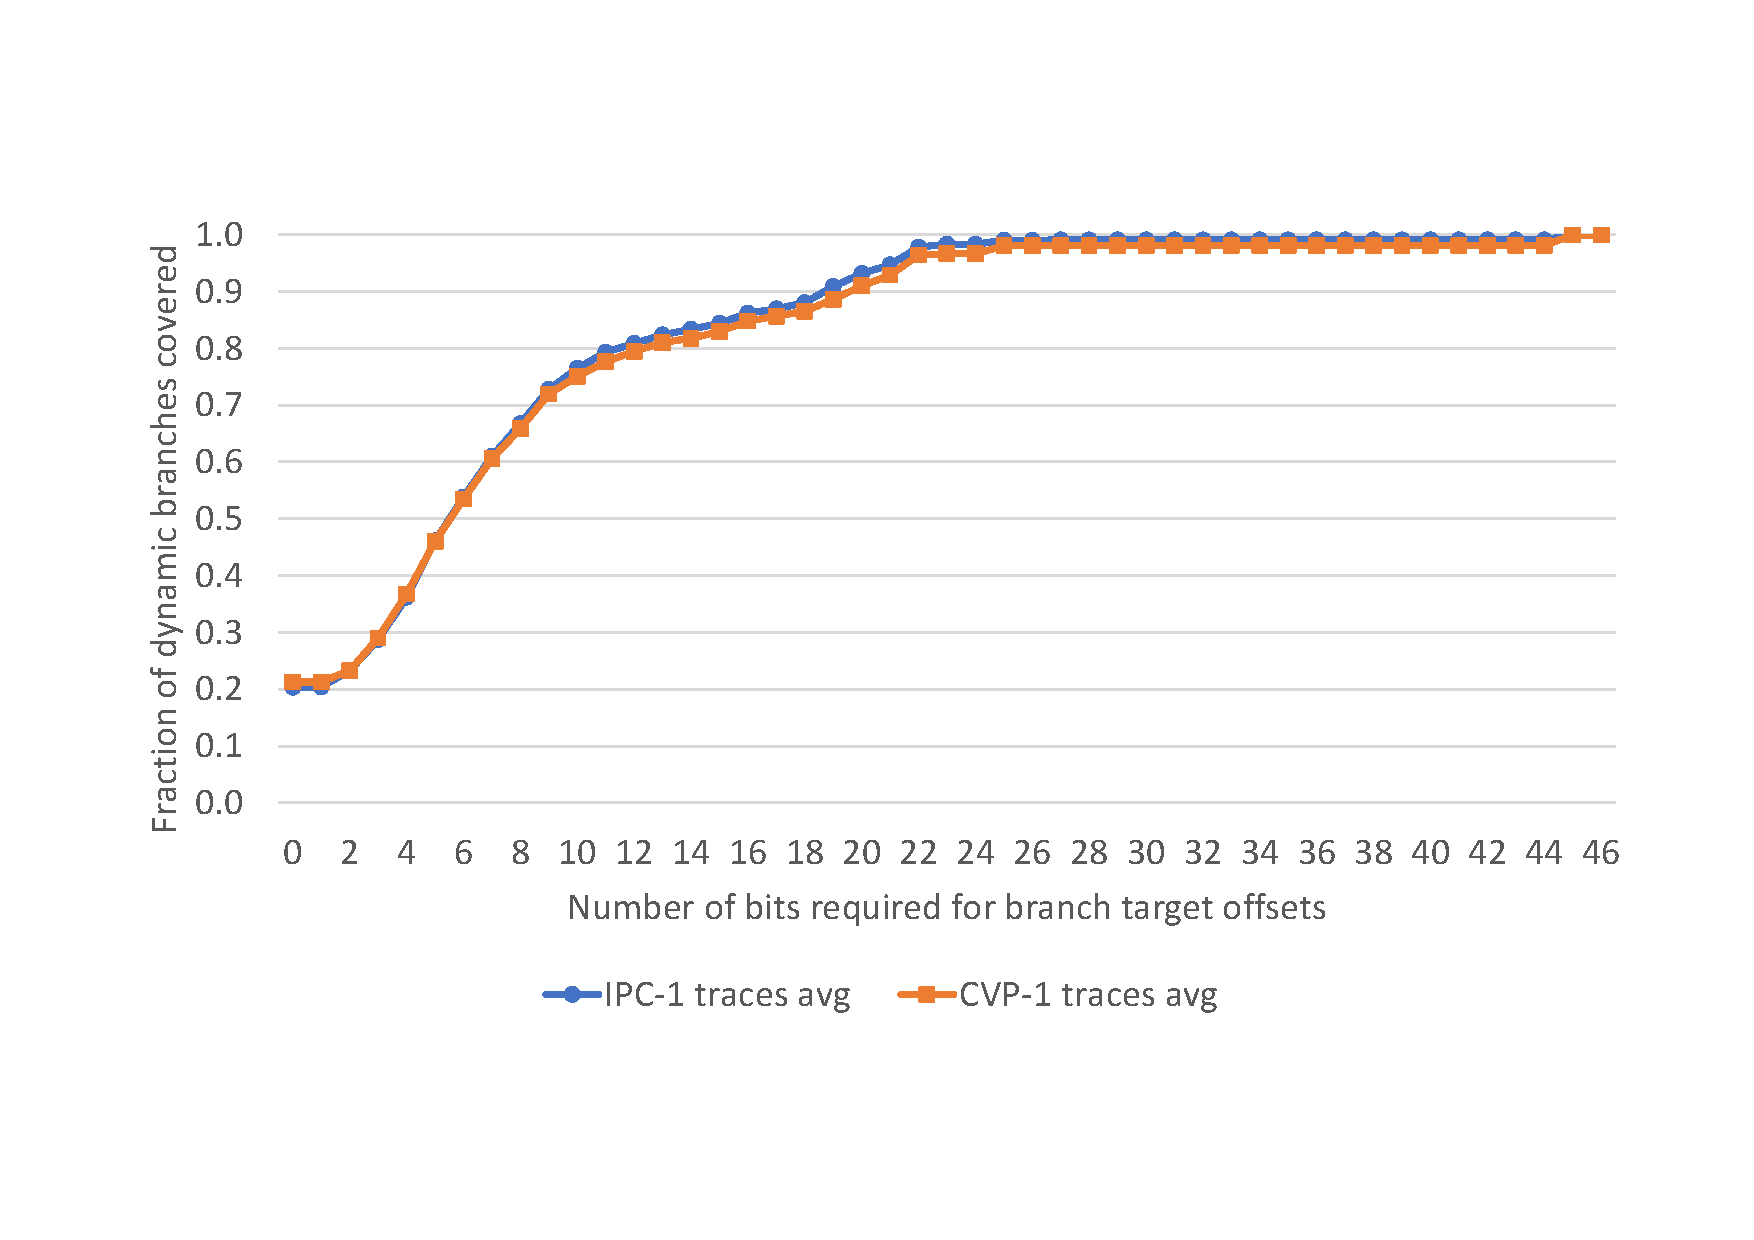
\includegraphics[width=\columnwidth, trim=70 90 60 100, clip]{figures/CVP-IPC.pdf}
%\vspace{-0.1in}
\caption{Target offset distribution in CVP-1 and IPC traces.}
\label{fig:cvp_res}
\end{figure}

We study the target offset distribution in 750+ Qualcomm server traces that were provided for the first Championship Value Prediction(CVP-1)~\cite{cvp}. The results, presented in \Cref{fig:cvp_res}, show that their offset distribution is very similar to the distribution in IPC-1 traces presented in \Cref{fig:offsets}. This study confirms that such an offset distribution is a consequence of how the applications are written and the resulting control-flow behavior. As discussed in \Cref{sec:analysis}, such offset distribution stems from the fact that the conditional branches dominate dynamic branch working set and they tend to have short offsets. This is because conditional branches guide the control-flow inside functions, and software engineering principles favor small functions. Consequently, short offsets dominate the branch offset distribution.

In addition to CVP-1 traces, we analyze five more server applications - Wordpress~\cite{wiki:wordpress}, Mediawiki~\cite{wiki:mediawiki}, and Drupal~\cite{wiki:drupal} from Facebook’s HHVM OSS-performance benchmarks~\cite{fboss}, Kafka~\cite{wiki:kafka} from Java DaCapo~\cite{blackburn2006dacapo}, and Finagle-HTTP~\cite{finagle-http} from Java Renaissance~\cite{Prokopec2019}. Further, these applications are compiled to x86 (CVP-1 and IPC-1 traces are compiled to Arm64) which also enables us to assess the impact of ISA on target offset distribution. The results presented in \Cref{fig:x86_res} show that the offset distribution in these applications is also very similar to that in IPC-1 traces. The only difference is that x86 traces require slightly larger offsets (1 or 2-bits more) to achieve a similar dynamic branch coverage as the Arm64 (CVP-1 and IPC-1) traces. For example, 6-bit offsets cover about 54\% branches in Arm64 traces, whereas x86 offsets need 8-bits to achieve 58\% branch coverage. This is because x86 offsets specify the distance between branch PC and target in number of \emph{bytes} because x86 instruction are variable size. In contrast, Arm64 offsets specify this distance in number of \emph{instructions} because all instructions are 4-bytes, thus saving 2 offset bits.

As BTB-X needs to store slightly larger offsets for x86 than Arm64, we reassess its storage advantage over PDede and Conv-BTB for x86 architectures. As each way in 8-way BTB-X needs to cover about 12.5\% of branches, we size its ways to store offset of 0-, 5-, 6-, 7-, 9-, 12-, 20-, and 27-bits based on the offset distribution in x86 applications shown in \Cref{fig:x86_res}. Thus, each set needs 86-bits for offsets compared to 80-bit in Arm64. Consequently, BTB-X's storage advantage is slightly lower for x86 than Arm64. However, BTB-X still stores 2.18x more branches than Conv-BTB for x86 (2.24x for Arm). Compared to PDede, BTB-X stores 1.21x more branches (1.24x for Arm64) at 0.9KB storage budget and 1.31x more branches (1.34x for Arm64) at 58KB storage budget. (\Cref{sec:storageBreak} presents this analysis of Arm64 traces.)

%\vspace{0.05in}

%\runinsec{Dynamically adjusting offset field size in BTB-X} BTB-X can be optimized to dynamically adjust offset field size to accommodate larger offsets if an application demands that. For example, we can merge the offset fields of neighboring entries to make space for larger offsets. This will require one bit per neighbor pair (7 bits in one 8-way set) to mark if a pair of neighboring entries is merged or not. We did not evaluate this optimization because the offset distribution in our traces does not diverge much from the average behavior.

\begin{figure}
\centering
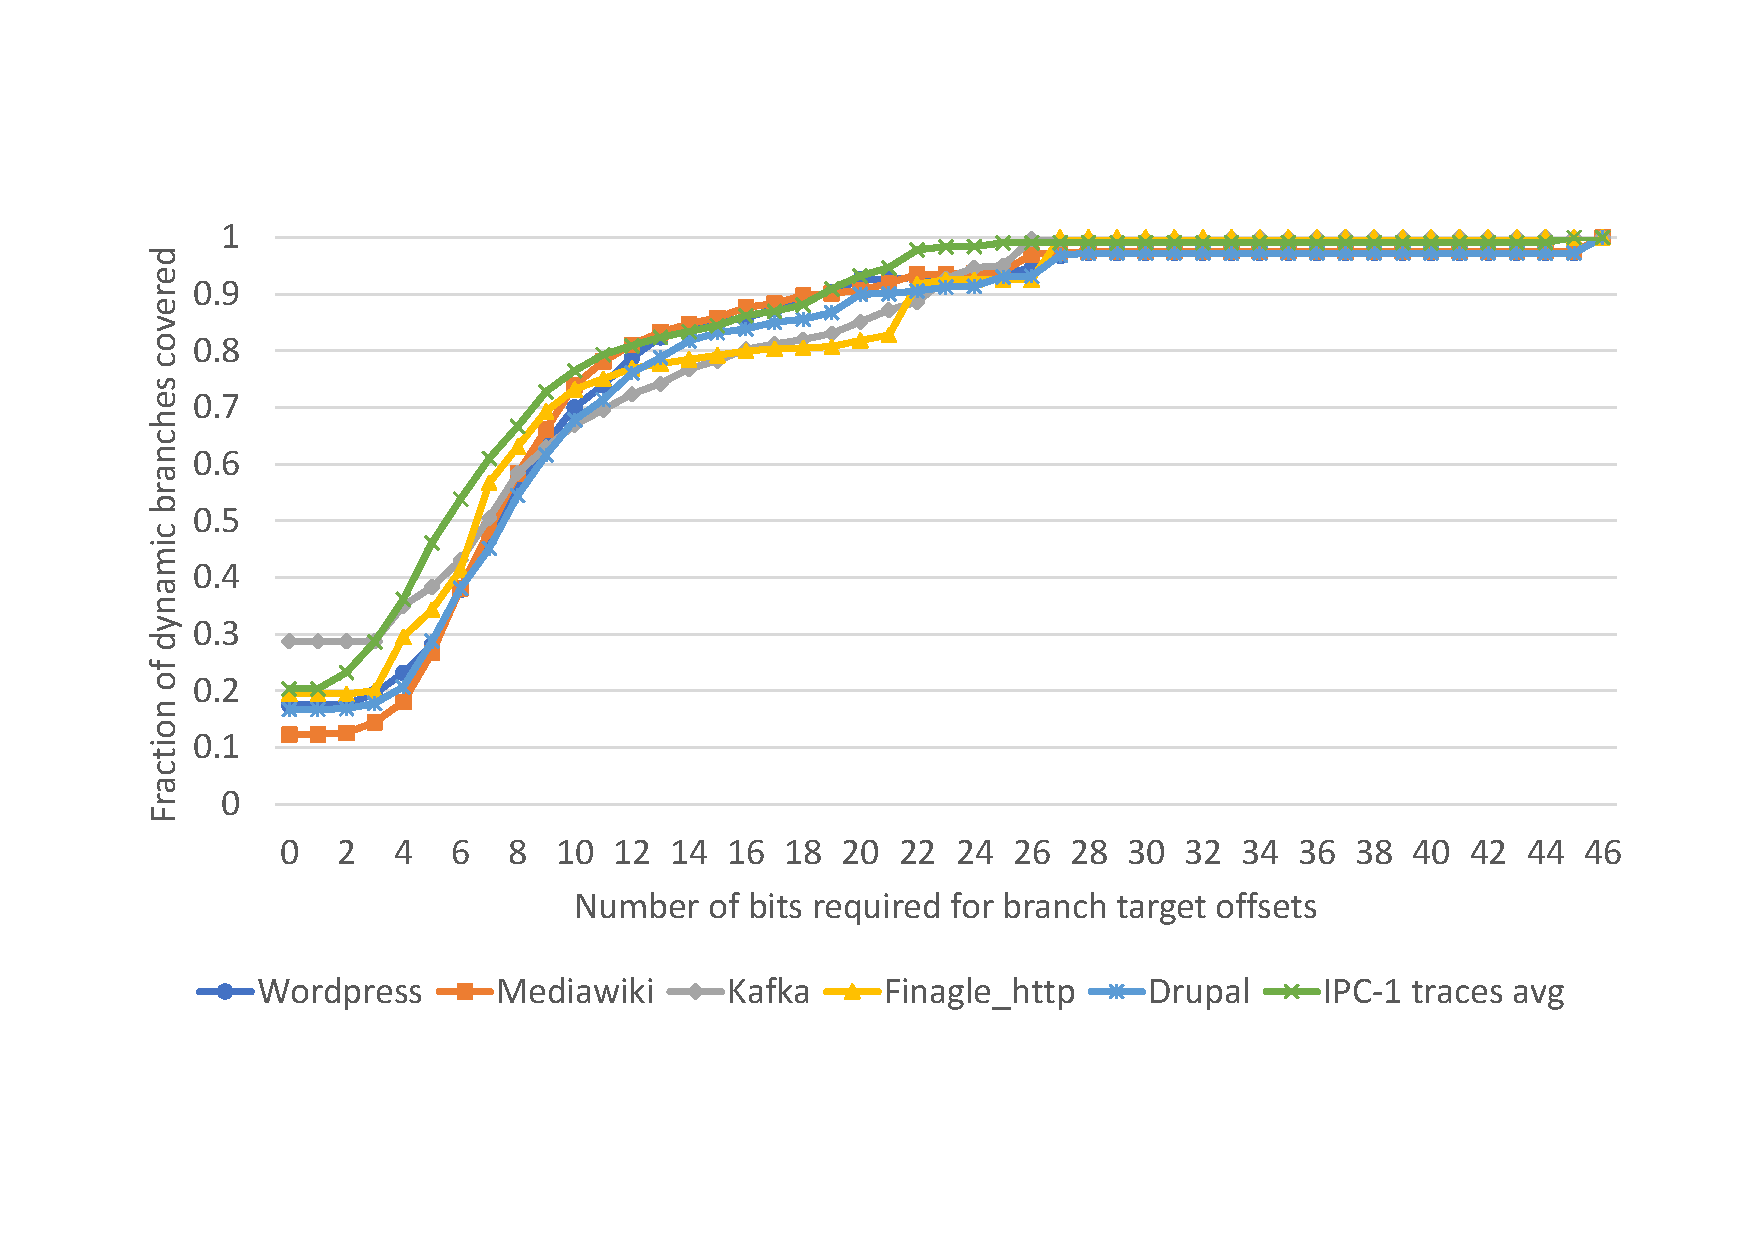
\includegraphics[width=\columnwidth, trim=70 90 60 100, clip]{figures/x86-IPC.pdf}
%\vspace{-0.1in}
\caption{Target offset distribution in x86 compiled server applications and Arm64 IPC traces.}
\label{fig:x86_res}
\end{figure}
